\chap{Magnetic Resonance}
This chapter is intended to give the reader a brief overview of the overwhelmingly large field that is nuclear magnetic resonance (NMR).\Nomenclature{NMR}{Nuclear Magnetic Resonance} The chapter introduces the quantum mechanical concept of spin but quickly moves on to describe magnetic resonance in terms of classical mechanics. Whereas it can be shown that many concepts touched upon in this thesis can equally well be described in terms of quantum phenomena, a measurement of the magnetic resonance signal does not make the spin ensemble collapse into a single particle eigenstate, hence motivating the adoption of a purely classical mechanical point of view~\cite{Hanson2008}.
\sect{Spin}
Spin is an intrinsic angular momentum present in all elementary particles. Elementary particles can be classified as either fermions or bosons. Fermions include quarks, leptons, and subatomic particles and nuclei composed of an odd number of quarks and leptons, such as protons and electrons. A common example of a boson would be the photon. All fermions have half-integer spin, i.e., the spin quantum number is an odd multiple of $1/2$ and are constrained by the Pauli exclusion principle that states that ``no two fermions can exist in identical quantum states''~\cite{Krane1988}. Spin gives rise to a magnetic dipole moment $\mu$ which is related to net spin angular momentum $\textbf{S}$ as
\begin{equation}
    \label{eq:spinmoment}
    \mu = \gamma\textbf{S}
\end{equation} where $\gamma$ is known as the gyromagnetic ratio. In the presence of an external static magnetic field, let us call it $B$, the magnetic dipoles will align themselves with the field in a precessing motion with the frequency
\begin{equation}
    \label{eq:larmor}
    \omega = \gamma B
\end{equation}
In magnetic resonance it often useful to consider a harmonic motion rather than an angular frequency, so the notation $\gbar = \frac{\gamma}{2\pi}$ is sometimes used. For a hydrogen nuclei, $\gammabar = 42.57$ MHz/T. The static field is often denoted $B_0$ and measured in Tesla, thus Eq.~\ref{eq:larmor} is often written as
\begin{equation}
    \omega_0 = \gamma B_0 \quad \textrm{or} \quad f_0 = \gbar B_0
\end{equation}
to denote the precession frequency when only a static magnetic field is present. Typical field strengths are $B_0 = 1.5$ T ($f_0 = 64$~MHz) and $B_0 = 3$ T ($f_0 = 128$~MHz).

In the quantum mechanical interpretation, alignment of the spins can be seen as a superposition of spin states. However, in the scope of this thesis, it is useful to consider the entire spin ensemble and its net magnetization, with corresponding net magnetization vector $\textbf{M} = (M_x, M_y, M_z)$~\cite{Levitt2001}. Due to thermal agitation and spin interactions the angular distribution of dipoles, the magnitude of $M$ at thermal equilibrium, denoted $M_0$ will be governed by a Boltzmann distribution, which predicts that
\begin{equation}
\label{eq:M0}
    M_0 = B_0\rho\frac{\gamma^2 \hbar^2}{4k_BT}
\end{equation}
where $\rho$ is the spin density, $\hbar$ is the reduced Planck constant, $k_B$ is Boltzmann's constant and T is the temperature in Kelvin.
\sect{Bloch equations}
The interaction between the net magnetization vector $\textbf{M}$ and a magnetic field $\textbf{B}$ can be described by the Bloch equation, which on a simplified form
can be expressed as
\begin{equation}
\label{eq:bloch1}
    \frac{d\textbf{M}}{dt} = \gamma(\textbf{M} \times \textbf{B})
\end{equation}
The simplification assumes that the orientation of $\textbf{M}$ is only due to the presence of an external magnetic field~\cite{Bloch1946}. At thermal equilibrium, the net magnetization only has a longitudinal component, i.e. $\textbf{M} = M_0(0, 0, 1)$. However, to be able to detect a signal, the net magnetization must be brought away from equilibrium, i.e. the spins need to be excited. This can be achieved by applying a time-varying magnetic field, let us call it $\textbf{B}_1(t)$, perpendicular to the static magnetic field $B_0$. The RF-field can be described as a \emph{linearly} polarized field
\begin{equation}
    \textbf{B}_1(t) = 2B_1^e(t)\textrm{cos}(\omega_{\textrm{rf}}\, t+\psi)\hat x
\end{equation}
where $B_1^e(t)$ is the pulse envelope function, e.g., a windowed sinc function, $\omega_{\textrm{rf}}$ is the carrier frequency and $\psi$ is the initial phase. In addition to the free precession about $B_0$, this will cause a forced precession of $\textbf{M}$ about $\textbf{B}_1(t)$. If the carrier frequency of $\textbf{B}_1(t)$ matches the Larmor precession frequency of the spins, know as the \emph{resonance condition}, it will cause the net magnetization vector to move in a spiral motion towards the transversal plane.

The linearly polarized field can be divided into two \emph{circularly} polarized fields
\begin{align}
  \textbf{B}_1(t) = B_1^e(t)\left(\textrm{cos}(\omega_{\textrm{rf}}\, t+\psi)\hat x - \textrm{sin}(\omega_{\textrm{rf}}\, t+\psi)\hat y \right) +
  \notag\\
     B_1^e(t)\left(\textrm{cos}(\omega_{\textrm{rf}}\, t+\psi)\hat x + \textrm{sin}(\omega_{\textrm{rf}}\, t+\psi)\hat y \right) \phantom{+}
\end{align}
where the first term is the resonant term which forces the precession, and the second term is an non-resonant term that only contributes to energy deposition. By using quadrature transmit coils, we can produce a circularly polarized field that only contains the resonant term
\begin{equation}
    \textbf{B}_1(t) = B_1^e(t)\left(\textrm{cos}(\omega_{\textrm{rf}}\, t+\psi)\hat x - \textrm{sin}(\omega_{\textrm{rf}}\, t+\psi)\hat y\right).
\end{equation}
As the frequency of the time-varying field typically resides in the radio frequency range, we refer to it as an RF-pulse. The angle between $\textbf{M}$ and the z-axis is characterized as the flip angle, and can be described as
\begin{equation}
    \label{eq:fa}
    \alpha = \gamma\int_0^\tau B_1^e(t)\,\dif t
\end{equation}
where $B_1^e(t)$ is the envelope function of effective field and $\tau$ is its duration~\cite{Bernstein2004}. Directly after the end of the RF-pulse, assuming the RF-pulse is applied along the positive $\hat x$ direction, the state of the system is as follows
\begin{equation}
	\textbf{B} =
	\begin{pmatrix}
		0\\0\\B_0\\
	\end{pmatrix}
\quad
\textrm{and}
\quad
	\textbf{M}(0) = M_0
	\begin{pmatrix}
		0\\\sin(\alpha)\\\cos(\alpha)\\
	\end{pmatrix},
\end{equation}
i.e. the only magnetic field present is the $B_0$ field along the z-axis and at time $t = 0$ the net magnetization has the magnitude which is equal to the magnitude of the equilibrium magnetization, denoted $M_0$, and forms an angle $\alpha$ to the transversal plane. The solution to Eq.~\eqref{eq:bloch1} is then
\begin{equation}
	\textbf{M}(t) = M_0
	\begin{pmatrix}
		\phantom{-}\cos(\omega_{0}\, t+\psi) \sin(\alpha) \\
		-\sin(\omega_{0}\, t+\psi) \sin(\alpha)\\
		\cos(\alpha) \\
	\end{pmatrix}
\end{equation}
which describes a precessing motion with the Larmor frequency. The transverse component, $\textbf{M}_{xy}$  can also be written in complex notation as
\begin{equation}
    M_{xy}(0) = M_0\sin(\alpha)\left( \cos(\omega_{0}\, t + \psi) - i\sin(\omega_{0}\, t + \psi) \right) = M_0\sin(\alpha)\, e^{-i\omega_{0}\, t}e^{-i \psi}
\end{equation}

To simplify the notation, a rotating frame of reference is often adopted, where the coordinate system rotates with the Larmor frequency. Figure~\ref{fig:blochplots_1} describes the process of excitation in both the static (laboratory) frame of reference and the rotating frame of reference.
\begin{figure}[htbp]
    \centering
    
\includegraphics[width=0.75\textwidth]{bloch_plot}
    \caption{The process of excitation can be visualized in both the laboratory frame of reference and the rotating frame of reference. The black arrow denotes the magnetization vector, and $\alpha$ denotes the flip angle.}
    \label{fig:blochplots_1}
\end{figure}
\sect{Relaxation}
In the previous section, we assumed that the orientation of $\textbf{M}$ was solely due to the presence of an external magnetic field $\textbf{B}_1$. However, there is also an interaction between the individual spins and the surrounding lattice, so-called \emph{spin-lattice} interactions, and interactions between spins with other spins, so-called \emph{spin-spin} interactions. These processes' will cause a loss of spin coherence in the transversal plane and regrowth of magnetization in the longitudinal plane in a process known as relaxation. The time constant that govern these two time courses are known as the \emph{spin-lattice relaxation time}, denoted $T_1$ and the \emph{spin-spin relaxation time}, denoted $T_2$. From Eq.~\ref{eq:larmor}, we can deduce that the precession frequency is dependent on the experienced magnetic field strength. This means that local variations in the magnetic field strength will cause spins to precess at slightly different frequencies, leading to a loss of coherence, and thus a loss of transverse net magnetization, which is different from the $T_2$-time. Therefore it is useful to define an ``apparent'' relaxation time, denoted $T_2^*$ defined as
\begin{equation}
    \label{eq:t2star}
    \frac{1}{T_2^*} = \frac{1}{T_2} + \frac{1}{T_2'}
\end{equation}
where $T_2'$ is the time constant that describes the loss of coherence that is attributed to local magnetic field variations. Depending on the type of pulse sequence used, the $T_2'$ effect may be negated, leaving the contrast to be affected only by $T_2$-relaxation. For the rest of this section, we will assume that the static magnetic field is homogeneous and that all loss of coherence can be attributed to $T_2$-relaxation.

As $T_1$ and $T_2$ relaxation are orthogonal processes (transversal and longitudinal) it is possible to decouple eq.~\ref{eq:bloch1} into two ordinary differential equations. Under the initial condition $\textrm{B} = (0,0,B_0)$ 
\begin{equation}
    \label{eq:decoupled_bloch_1}
    \frac{dM_z}{dt} = 0
\end{equation}
\begin{equation}
    \label{eq:decoupled_bloch_2}
    \frac{\dif\textbf{M}_{xy}}{\dif t} = \gamma ( \textbf{M}_{xy}\times \textbf{B})
\end{equation}
It's was previously stated in Eq.~\ref{eq:bloch1} that \textbf{M} was only affected by the presence of an external magnetic field, but from the previous discussion it's clear that this assumption does not hold, and subsequently Eq.~\ref{eq:bloch1} must be modified accordingly. As already described, the longitudinal growth rate is proportional to the difference between $M_0$ and $M_z$ by the proportionality constant $T_1$, meaning that Eq.~\ref{eq:decoupled_bloch_1} can be restated as
\begin{equation}
    \frac{\dif M_z}{\dif t} = \frac{1}{T_1}(M_0-M_z)
\end{equation}
which has the solution
\begin{equation}
    M_z(t) = M_z(0)e^{-t/T_1} + M_0(1-e^{-t/T_1})
\end{equation}
The transversal decay can be described by saying that $M_{xy}$ decreases by the time constant $T_2$, i.e. Eq.~\ref{eq:decoupled_bloch_2} is restated as
\begin{equation}
    \frac{\dif \textbf{M}_{xy}}{\dif t} = \gamma ( \textbf{M}_{xy}\times \textbf{B}) - \frac{1}{T_2}\textbf{M}_{xy}.
\end{equation}
Assuming that \textbf{B} is not time-dependent, i.e. that no RF-pulse is present, the solution can be written as
\begin{equation}
    M_{xy}(t) = M_{xy}(0)e^{-t/T_2}.
\end{equation}
Finally, we arrive at an expression for the magnetization after an RF-pulse with flip angle $\alpha$, considering relaxation, which can be described as
\begin{equation}
    M_z(t) = M_0\,\textrm{cos}(\alpha)e^{-t/T_1} + M_0(1-e^{-t/T_1})
\end{equation}
\begin{equation}
    M_{xy}(t) = M_0\,\textrm{sin}(\alpha)e^{-t/T_2}\,e^{-i\omega_{0}\,t}e^{-i\psi}
\end{equation}
\begin{figure}[hbtp]
    \begin{subfloat}
        \centering
        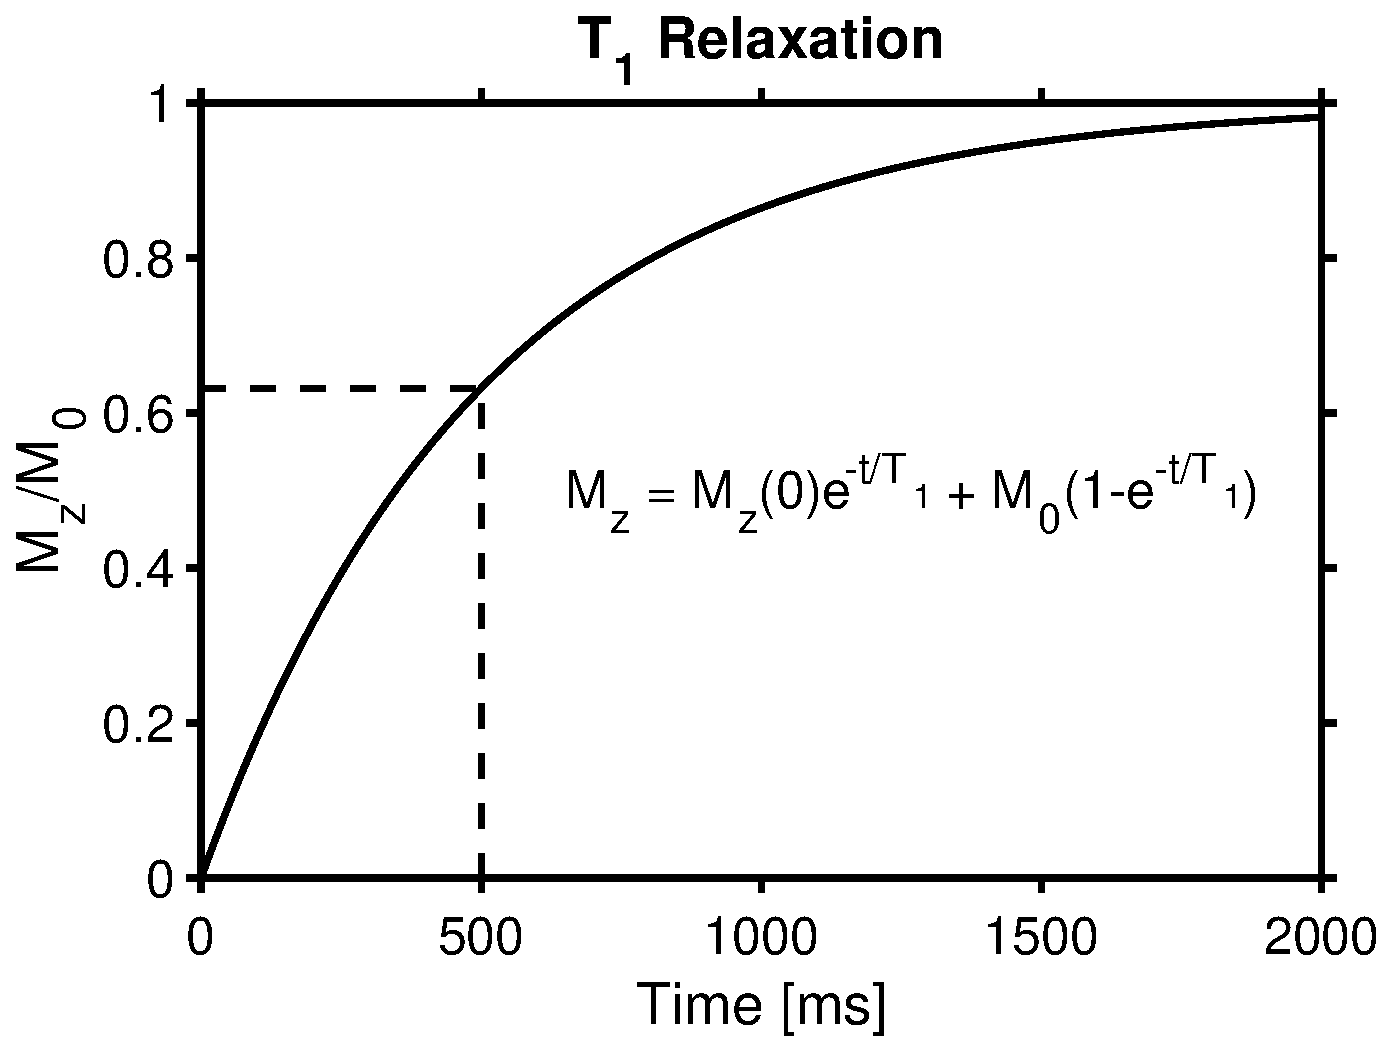
\includegraphics[width=0.49\textwidth]{t1}
    \end{subfloat}
    \begin{subfloat}
        \centering
        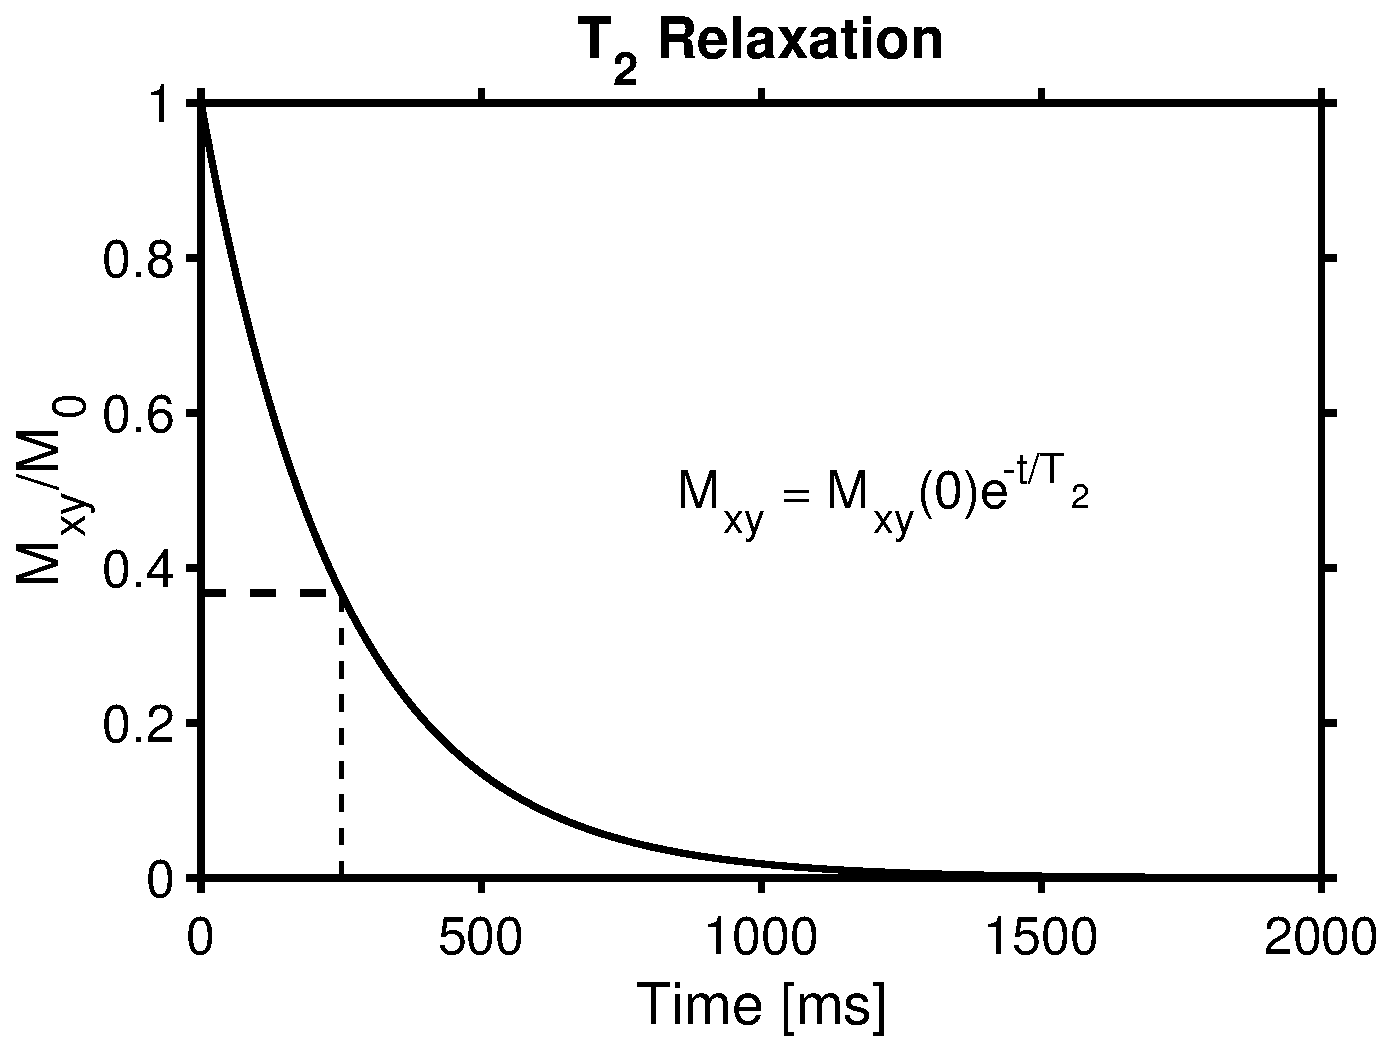
\includegraphics[width=0.49\textwidth]{t2}
    \end{subfloat}
    \caption{Bloch equation simulations of $T_1$ decay (left) and $T_2$ decay (right). The time constant $T_1$ is defined as the time at which $63\%$ of the longitudinal magnetization is recovered ($1-e^{-1} = 0.6321$) and $T_2$ is defined as the time when $37\%$ of the transversal magnetization remains ($e^{-1} = 0.3679)$. The simulation parameters were as follows: $T_1 = 500\textrm{ ms}, T_2 = 250\textrm{ ms}$, $M_z(0) = 0$, and $M_{xy}(0) = M_0$ }
    \label{fig:relaxation}
\end{figure}
\sect{Signal reception}
To receive a signal, we use sensitive receiver coils. The transverse magnetization will create a voltage in the receiver coils, in accordance with Faraday's law of induction
\begin{equation}
    V(t) = -\frac{\partial \Phi}{\partial t} = -\frac{\partial}{\partial t}\int_{\textrm{object}} \textbf{B}(\textbf{r})\cdot\textbf{M}(\textbf{r},t) \dif \textbf{r}
\end{equation}
where $\Phi$ is the magnetic flux, $\textbf{B}$ is the receiver coil sensitivity and $\textbf{r}$ is the location in space. By assuming a uniform sensitivity, calculating the partial derivative, and performing some simplifications we arrive at
\begin{equation}
    V(t) = -\int_{\textrm{object}} \omega(\textbf{r})M_{xy}(\textbf{r},0)e^{-t/T_2}\cdot\sin(-\omega(\textbf{r})t + \psi(\textbf{r}))\,\dif\textbf{r}
\end{equation}
The MR scanner uses what is know as phase sensitive detection. The voltage measured by the coil is demodulated by a sine and a cosine function which is on-resonance with the Larmor frequency, then low-pass filtered to obtain what is essentially the rotating frame of reference signal. In complex notation, the measured, demodulated, signal can be expressed as
\begin{equation}
    S(t) = \omega_0e^{i\pi/2}\int_{\textrm{object}}M_{xy}(\textbf{r},0)e^{-t/T_2(\textbf{r})}e^{-i\Delta \omega(\textbf{r})t}\dif \textbf{r}
    \label{eq:signal}
\end{equation}


%To excite and receive the signal, we use coils. One specific coil setup can be used for transmission (TX) \Nomenclature{TX}{Transmission} or for reception (RX), \Nomenclature{RX}{Reception} or both (TX/RX). The bird-cage "body coil" built into the bore of the MR scanner is a so called TX/RX-coil meaning that it can both be used both to excite the spins, and to receive signal. The body coil has a large reception volume, with a very uniform signal, albeit with a low signal-to-noise ratio (SNR). \Nomenclature{SNR}{Signal-to-noise ratio} Instead, phased array surface coils can be used to receive a signal with high SNR, but with an non-uniform reception field~\cite{Roemer1990}.

\sect{Free Induction Decay}
If a signal is acquired from the moment the excitation pulse was turned off, and until the signal had naturally decayed, one would obtain what is known as a free induction decay (FID) \Nomenclature{FID}{Free induction decay}~\cite{Hahn1953}. The FID would contain all signals in the imaging volume superimposed on each other. Using the FID, one could apply the inverse Fourier transform to obtain a frequency spectrum, representing the molecular content of the sample volume. Depending on the molecular makeup of the sample, several peaks might be visible, as the resonant frequency depends on the molecular environment of the protons, and in particular, the number of electrons shielding the nucleus. The Larmor frequency is sometimes expressed as
\begin{equation}
    \omega_0 = \gamma B_0(1-\sigma)
    \label{eq:larmor_shield}
\end{equation}
where $\sigma$ is the shielding constant. The difference is resonant frequency is called chemical shift, denoted $\delta$, and is measured in parts per million (ppm). The difference between water and fat, for instance, is about 3.5 ppm~\cite{Harris2001}.

\sect{Gradients and spatial encoding}
To create an image from the acquired signal, the MR signal must be spatially encoded. This is achieved by superimposing spatially variant gradient field over the static magnetic field $B_0$, such that $B = B_0 + \textbf{G}$, where the gradient field $\textbf{G} = (G_x,G_y,G_z)$ can be described as 
\begin{equation}
    G_x = \frac{\dif B}{\dif x}, \quad G_y = \frac{\dif B}{\dif y}, \quad G_z = \frac{\dif B}{\dif z}. 
\end{equation}

The last exponential term in Eq.~\ref{eq:signal} represents the spatial variation precession frequency. This can be defined as
\begin{equation}
    \Delta \omega(\textbf{r})\,t = \gamma\textbf{G}\cdot\textbf{r} = 2\pi\textbf{k}\cdot\textbf{r}.
\end{equation}
Instead of angular frequencies $\omega$, we introduce $\textbf{k}$ as a representation spatial frequencies, where
\begin{equation}
    \textbf{k}(t) = \gbar\int_0^t \textbf{G}(\tau)\,\dif\tau
\end{equation}

This formalism is the foundation of what is known as the k-space~\cite{Twieg1983, Ljunggren1983}. The k-space can be seen as the Fourier transform of the image. The k-space has an inverse relationship with the image, e.g., the sampling distance in k-space ($\Delta k$) is proportional to the field of view \Nomenclature{FOV}{Field of view}(FOV) 
\begin{equation}
    \Delta k = \frac{1}{\textrm{FOV}}
\end{equation}
and the extent of the k-space is related to the resolution in image space,
\begin{equation}
    \Delta w = \frac{1}{2\, k_{\textrm{max}}}
\end{equation}
where $\Delta w$ is the voxel size in k-space, assuming a k-space extent of $\pm k_{\textrm{max}}$, see Figure~\ref{fig:kspace}.
\begin{figure}[htbp]
    \centering
    \includegraphics[width=\textwidth]{kspace2}
    \caption{The magnitude of the k-space, in logarithmic scale (left) and the magnitude of the corresponding image (right). The inverse Fourier transform is used to transform between the k-space and the image space. \emph{Note:} The size of $\Delta k$ and $\Delta w$ are exaggerated for clarity.}
    \label{fig:kspace}
\end{figure}

Three types of spatial encoding are commonly used
\begin{itemize}
    \item Slice selection
    \item Phase encoding
    \item Frequency encoding
\end{itemize}

For the sake of this discussion, we assume that slice selection is made along the $z$-direction, phase encoding along the $y$-direction, and frequency encoding along the $x$-direction.
\subsect{Slice selection}
Only spins with a precession frequency $\omega$ that matches the carrier frequency $\omega_{\textrm{rf}}$  of $\textbf{B}_1$ will be excited. By applying a gradient along the z-axis, the selected slice will be at the position
\begin{equation}
    z = \frac{\omega - \gamma B_0}{\gamma G_z}
\end{equation}
in relation to the isocenter.
\subsect{Phase encoding}
The phase encoding gradient is switched on for a time $\tau$ along the phase encoding direction. During this time, spins will precess with different frequencies, resulting in a linear phase difference at the time when the phase encoding gradient is turned off. This phase difference can be described as
\begin{equation}
    \phi(x,y) = \gamma G_y \tau y
\end{equation}
\subsect{Frequency encoding}
During the signal acquisition, a gradient will be switched on creating a linear difference in precession frequency, which can be described as
\begin{equation}
    \omega(x,y) = \gamma G_x x
\end{equation}

%\sect{Magnetic Resonance Imaging}
%The concept of NMR was initially used as non-invasively measure the magnetic properties of samples, such as the magnetic moment~\cite{Rabi1938} or the relaxation time~\cite{Hahn1949}. However, in 1973 Lauterbur paved the way for magnetic resonance imaging with his seminal paper on using local magnetic field gradients to form an image~\cite{Lauterbur1973}.
\sect{Pulse sequences}
The order and timing in which the RF-pulses and gradients are played out is referred to as a pulse sequence. The pulse sequences can roughly be divided into two families; spin echo and gradient echo. The difference is how the \emph{echo} is formed. In a spin echo sequence, the echo is formed by applying a refocusing $180^\circ$ RF-pulse at $\textrm{TE}/2$, whereas gradient echo relies on the gradients alone to form the echo. A major difference between the two is that in a gradient echo pulse sequence, the transversal magnetization will experience $T_2^*$ decay, where the refocusing pulse of a spin echo pulse sequence would cancel out the $T_2'$ effects, leaving the transversal magnetization affected by $T_2$ alone.

For the rest of this thesis, only gradient echo pulse sequences will be considered. A common example of a gradient echo pulse sequence is Fast Low Angle Shot (FLASH) \Nomenclature{FLASH}{Fast low angle shot}. The sequence is executed with a low flip angle, and a short TR which is finished by a spoiler to dephase any residual magnetization before the next excitation. The signal equation for a FLASH sequence is given by
\begin{equation}
    S \propto \frac{\sin(\alpha)(1-e^{-\textrm{TR}/T_1})}{1-\cos(\alpha)\,e^{-\textrm{TR}/T_1}}e^{-\textrm{TE}/T_2^*}
    \label{eq:flash}
\end{equation}
By taking the partial derivative of S with respect to $\alpha$, the optimal flip angle for a FLASH sequence, sometimes known as the Ernst angle \cite{Ernst1966}, is found to be
\begin{equation}
    \alpha = \textrm{acos}\left ( e^{-\textrm{TR}/T_1} \right ).
\end{equation}
A schematic example of a gradient echo pulse sequence can be seen in Figure~\ref{fig:gre}.
\begin{figure}[htbp]
    \centering
    \includegraphics[width=\textwidth]{gre2}
    \caption{A schematic diagram of a gradient echo pulse sequence (left). The shaded box indicates one repetition. The RF pulse envelope in this example is a Hamming windowed sinc function, designed using John Pauly's RF design toolbox~\cite{Pauly1991}. In this figure, the gradient spoilers are omitted for brevity. A representation the k-space trajectory (right). The gray dotted line denotes the effect of the phase encoding gradient and the readout prewinder. The black dotted line denotes the readout of one k-space line.}
    \label{fig:gre}
\end{figure}
\sect{bSSFP}
The concept of Steady State Free Precession (SSFP, also known as FISP or FFE) \Nomenclature{SSFP}{Steady State Free Precession} \Nomenclature{FISP}{Fast imaging with steady state precession} \Nomenclature{FFE}{Fast field echo} predates magnetic resonance imaging. The concept was introduced as method to improve signal-to-noise ratio (SNR)\Nomenclature{SNR}{Signal-to-noise ratio} of NMR-measurements~\cite{Carr1958}. In the seminal paper, it's noted to have properties similar to that of a spin echo~\cite{Hahn1950}. In imaging, the SSFP method is often used with balanced gradients over one TR, i.e. the TE $= 2\,$ TR, and the gradient moment is nulled over one TR. In these cases, the sequence is referred to as balanced SSFP (bSSFP), TrueFISP, FIESTA \Nomenclature{FIESTA}{Fast imaging employing steady state acquisition} or balanced-FFE. \Nomenclature{bSSFP}{Balanced Steady State Free Precession} The bSSFP signal comprises both gradient echos, spin echoes and stimulated echos~\cite{Scheffler2003a,Scheffler2003b}. Compared to the FLASH method, bSSFP uses much higher flip angles, which may lead to more patient heating~\cite{Srinivasan2015}.

The signal equation for bSSFP can be expressed as
\begin{equation}
    S \propto \frac{\sin(\alpha)(1-e^{-\textrm{TR}/T_1})e^{-\textrm{TE}/T_2}}{1-(e^{-\textrm{TR}/T_1}-e^{-\textrm{TR}/T_2})\cos(\alpha)-(e^{-\textrm{TR}/T1})(e^{-\textrm{TR}/T_2})}
    \label{eq:bssfp1}
\end{equation}
In bSSFP, $\textrm{TE} = 2\,\textrm{TR}$, so it's usually safe to assume that $\textrm{TR} \ll T_1$. This means that we can disregard any TR-dependence, and subsequently simplify the equation to
\begin{equation}
    S \propto \frac{\sin(\alpha)e^{-\textrm{TE}/T_2}}{1+\cos(\alpha)+(1-\cos(\alpha))(T_1/T_2)}
    \label{eq:bssfp2}
\end{equation}
From Eq.~\ref{eq:bssfp2} it is apparent that the contrast is dependent on the ratio $T_2/T_1$~\cite{Huang2002}. This contrast weighting have been proven useful in cardiovascular imaging, where it provides a strong contrast between myocardium and blood~\cite{Caudron2011, Bieri2013}. 
\begin{figure}
    \centering
    \includegraphics[width=0.75\textwidth]{bssfp_sequence}
    \caption{The gradient echo pulse sequence diagram from Figure~\ref{fig:gre} is here modified to describe a balanced steady state free precession pulse sequence. Note the addition of the balancing gradients that nulls the gradient moment on each axis over the repetition time, indicated by the shaded box. Note: This is a schematic representation of the pulse sequence diagram, and some gradients may not be to scale.}
    \label{fig:bssfp}
\end{figure}
Similar to the gradient echo method previously discussed, bSSFP is a steady-state method. To establish steady state as rapidly as possible, a preparatory ``$\alpha/2-\textrm{TR}/2$''-module is often used where only half of the flip-angle and half the repetition time is used in the first repetition~\cite{Deiming1994:ISMRM}. Figure~\ref{fig:blochplots_2} shows the transient steady-state when an ``$\alpha/2-\textrm{TR}/2$''-module is properly executed, and what happens when the magnetization is not properly prepared. An alternative approach is to use a ramp of linearly increasing RF-pulses~\cite{Nishimura2000:ISMRM, Deshpande2003} or a Kaiser-windowed ramp~\cite{LeRoux2003}.
\sect{Eddy currents in bSSFP}
Any imaging sequence will be affected by eddy currents, however in bSSFP, these effects take on a particular appearance. In the bSSFP method the RF-pulse phase is incremented by $180^\circ$ prior to each excitation. Assuming that the phase accrual is constant from TR to TR, a transversal steady state can be established over a $2 \textrm{TR}$ phase cycle, in addition to the longitudinal steady-state that is common to other gradient echo based methods. If this phase cycle is perturbed it may induce long-lived oscillations in the steady state signal. Figure~\ref{fig:blochplots_3} demonstrates what happens when a small phase perturbation is introduced into the bSSFP signal. Such phase perturbations can also come from other sources, such as flow \cite{Lagerstrand2009}, with similar effects on the steady state signal.
\begin{figure}
    \centering
    \includegraphics[width=\textwidth]{bieri1}
    \caption{Bloch-simulated time evolution during transient steady-state. The readout is initiated using an $\alpha/2-\textrm{TR}/2$ magnetization preparation (left) and without a shortened repetition time (right). The dashed line denotes the signal evolution off resonance ($30^\circ/\ \textrm{TR}$) and the solid line the signal evolution on resonance ($0^\circ/\ \textrm{TR}$). The simulation parameters were as follows: $\textrm{TE}/ \textrm{TR} = 1.75/3.5$ ms, $ \textrm{T}_1 = 140$ ms, $\textrm{T}_2 = 70$ ms, $\alpha = 70^\circ$. The right image is adapted from~\cite{Bieri2005a}.}
    \label{fig:blochplots_2}
\end{figure}
\begin{figure}
    \centering
    \includegraphics[width=\textwidth]{bieri2}
    \caption{Bloch-simulated time evolution at a stable steady-state (left), and with an initial phase perturbation of $1^\circ$ at time = 0 TR (right). The dashed line denotes the signal evolution off resonance ($30^\circ/\ \textrm{TR}$) and the solid line the signal evolution on resonance ($0^\circ/\ \textrm{TR}$). The simulation parameters were the same as in Figure~\ref{fig:blochplots_2}. Images are adapted from~\cite{Bieri2005a}.}
    \label{fig:blochplots_3}
\end{figure}

\sect{Radial imaging}
Conventionally, k-space is sampled on a Cartesian grid. However, the very first MR imaging method was based on projection imaging, similar to computed tomography \cite{Lauterbur1973}. By rotating the readout gradient in the physical coordinate system, a projection of the object was obtained. In the trajectory formalism, this can be likened to reading radial lines through the center of k-space. These radial lines are often referred to as spokes. The reconstruction of radial images generally requires an extra step compared to Cartesian image reconstructions. The non-Cartesian k-space cannot readily be transformed to image space using the fast Fourier transform algorithm (FFT), \Nomenclature{FFT}{Fast Fourier transform} which requires uniformly spaced sampling points. A common solution is to ``regrid'' the data onto a uniform grid, either through linear interpolation, or using a convolution kernel~\cite{Jackson1991}, see Figure~\ref{fig:gridding}. Two alternative methods are to calculate a non-uniform Fourier transform~\cite{Sarty2001}, or to use GRAPPA weights for the interpolation of the sampling points~\cite{Seiberlich2007}.
\begin{figure}[htbp]
    \centering
    \includegraphics[width=\textwidth]{gridding}
\caption{A schematic overview of grid-driven (left) and data-driven (right) interpolation of sampling points onto a rectilinear grid. In the grid-driven approach, the value at each grid point (crosses) is found using bi-linear interpolation of the adjacent radial sample points (solid circles). In the data-driven approach, each radial sampling point is distributed onto the grid using kernel interpolation (dashed circle).}
    \label{fig:gridding}
\end{figure}
Using radial sampling, the density of the sampling points will be highest in the middle and decrease as a function of distance. A common approach is to use a linear ramp, or a Ramachandran-Lakshminarayanan (Ram-Lak) filter~\cite{Ramachandran1971}, to make the k-space density more uniform. However, for high undersampling factors, or for highly non-uniform k-space distributions, linear methods may not be sufficient. As an alternative, iterative methods based on gridding the trajectory have been proposed~\cite{Pipe1999}, see Figure~\ref{fig:pipe}. Analytical approximations have also been proposed~\cite{Nielles-Vallespin2007}. 
\begin{figure}
    \centering
    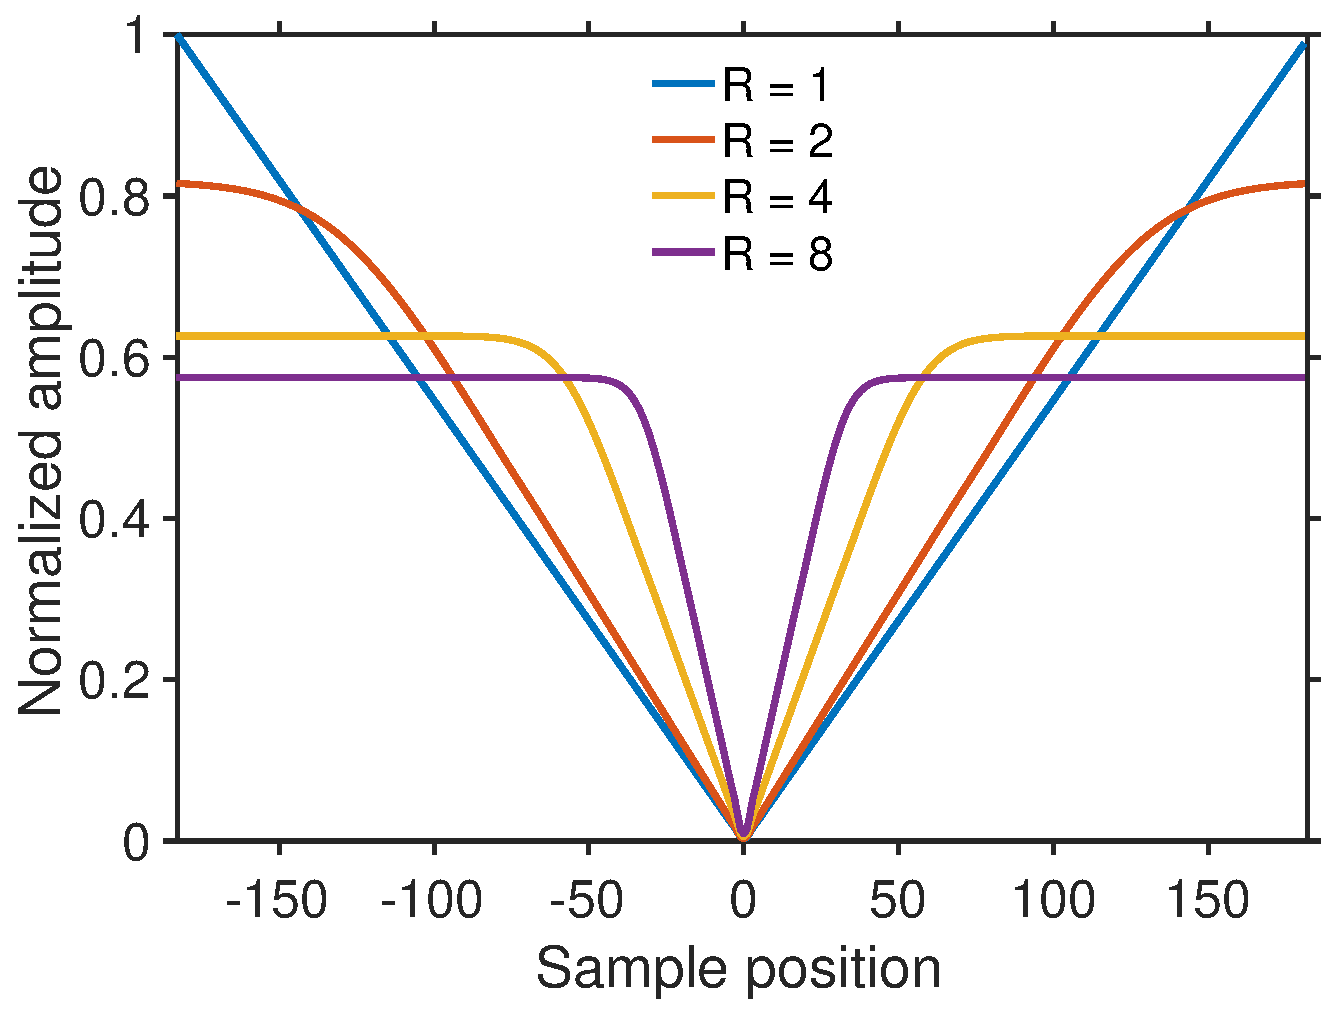
\includegraphics[width=0.65\textwidth]{dcf_pipe}
\caption{Optimized k-space density weighting filters, for a range of undersampling factors, calculated using iterative gridding of the sampling trajectory.}
    \label{fig:pipe}
\end{figure}

\sect{Image reconstruction}
To go from k-space to image space, the Fourier transform is used. However, direct reconstruction of images requires that the sample points are equidistant and that the Nyquist-Shannon sampling theorem is fulfilled in every part of k-space. Violating the Nyquist-Shannon will result in aliasing artifacts. In Cartesian imaging, the aliasing artifacts manifest as ``fold-over'' artifacts where parts of the images is folded back onto itself. The sampling theorem can also be violated on purpose in order to acquire the image faster. By exploiting the variation in spatial sensitivity, \emph{parallel imaging} methods can be used to undo the aliasing, either directly in k-space using GRAPPA \cite{Griswold2002} and SPIRiT \cite{Lustig2010}, or in the image using SENSE \cite{Pruessmann1999}. Many of these methods can be applied to non-Cartesian sampling as well \cite{Wright2014}, such as Radial-GRAPPA \cite{Seiberlich2008, Seiberlich2011} and CG-SENSE \cite{Pruessmann2001}.

\sect{Phase~contrast MRI}
Phase~contrast MRI can be seen as an extension of flow compensation. In MRI, motion is related to phase. 
Phase~contrast~MRI~\cite{Moran1982, Moran1985} measures the velocity of moving spins by making use of the fact that MRI is an inherently phase-sensitive measurement method. The acquired phase due to a static spin with a gradient $G(t)$ is linearly dependent to the 0th gradient moment
\begin{equation}
    M_0 = \gamma \int_0^\tau G(t)\,\dif t
\end{equation}
whereas the phase acquired by spin moving with a constant velocity is dependent on both the 0th the 1st gradient moment,
\begin{equation}
    M_1 = \gamma \int_0^\tau G(t)t\,\dif t. 
\end{equation}
A spin moving with a velocity $v$ will therefore acquire the phase
$\phi = M_0 + v\, M_1$. A phase~contrast image is created by acquiring images encoded with two different $M_1$ values at the echo, encoding A and encoding B \cite{VanDijk1984,Bryant1984}. By subtracting encoding A and B, only the phase due to moving spins is left. In analogy to how the frequency encoding was described in k-space, we can also speak of a velocity k-space value
\begin{equation}
    k_v = \gamma M_1
\end{equation}
An important parameter in phase~contrast MRI is the velocity encoding strength, VENC, which is defined as
\begin{equation}
    \textrm{VENC} = \frac{\pi}{k_v}
\end{equation}
Flow with velocity $\pm$VENC will acquire a phase of $\pm\pi$, whereas higher velocities will experience aliasing, see Figure~\ref{fig:venc}.
\begin{figure}[htbp]
    \centering
    \includegraphics[width=0.75\textwidth]{img/pc3-01.eps}
\caption{The gradient echo pulse sequence diagram from Figure~\ref{fig:gre} has been modified into a phase~contrast pulse sequence with through-slice velocity encoding. Note the addition of flow compensation and bipolar velocity encoding gradients. The solid bipolar gradient pair indicates encoding A, and the dashed gradients indicate encoding B. Note: This is a schematic representation of the pulse sequence diagram, some gradients may not be to scale. Gradient spoilers were omitted for brevity.}
    \label{fig:pc2}
\end{figure}
\begin{figure}[htbp]
    \centering
    \includegraphics[width=\textwidth]{C14_rev_2_copy.png}
\caption{Illustrative examples of velocity encoded images with VENC = 30 cm/s. Note the aliasing in the left ventricle which is visible as a distinct border between black and white. }
    \label{fig:venc}
\end{figure}
